
%----------------------------------------------------------------------------
\chapter{Interval Abstraction}
\label{sec:intervalabstraction}
%----------------------------------------------------------------------------

%----------------------------------------------------------------------------
\section{Library}
%---------------------------------------------------------------------------- 

\begin{definition}{Bound}
	A Bound is a specified whole number or Infinite (can be positive or negative) $Bound \in \mathbb{Z} \lor Bound \in \{ +\infty, -\infty \}$
\end{definition}

\begin{definition}{max($Bound1$, $Bound2$)=}

	if $Bound1 == +\infty \lor Bound2 == +\infty$ then $+\infty$
	
	else if $Bound1 == -\infty \lor Bound1<Bound2$ then $Bound2$
	
	else $Bound1$	
\end{definition}

\begin{definition}{min($Bound1$, $Bound2$)=}

if $Bound1 == -\infty \lor Bound2 == -\infty$ then $-\infty$

else if $Bound1 == +\infty \lor Bound1>Bound2$ then $Bound2$

else $Bound1$	
\end{definition}

\begin{definition}{$Bound+K \in \mathbb{Z}$)=}
	
	if $Bound == +\infty \lor Bound == -\infty$ then $Bound1$
	
	else ($Bound \in \mathbb{Z}$) then $Bound+K$
\end{definition}

\begin{definition}{$|Bound|$=}
	
	if min($Bound$, $0$) $==0$ then $Bound$
	
	else $Bound*(-1)$
\end{definition}
	
	Or
	
\begin{definition}{$|Bound|$=}
	
	if $Bound \in  \mathbb{Z}$ then $|Bound|$ is the regular $absolute function$ in $\mathbb{Z}$
	
	else $|Bound| = +\infty$
\end{definition}

\begin{definition}{Interval}
	An interval is specified with two Bounds: the lower Bound($LB$) and the higher Bound($HB$).
	
	ex.: $(2;+\infty)$, $(3;1)$
\end{definition}

\begin{definition}{Interval is valid}
	
	if min($LB$, $HB$) == $LB \neq +\infty \land$ max($LB$, $HB$) == $HB  \neq -\infty$
	
	Note: empty interval ($Ei$) $\equiv$ invalid interval
	
	Note2: intervals $(+\infty, +\infty)$, $(-\infty, -\infty)$ are also empty intervals 
	
	ex.: $(2;+\infty)$ and $(0;0)$ is valid, but $(3;1)$ is not valid $\equiv$ invalid
\end{definition}

\begin{definition}{section of two intervals $Interval1 \cap Interval1$=}
	
	if $Interval1, Interval2$ is valid then 
	
	$LB$=max($Interval1.LB$, $Interval2.LB$)
	
	$RB$=min($Interval1.HB$, $Interval2.HB$)
	
	else $Ei$
	
	ex.: $(2,8)\cap(1,3)=(2,3)$, $(2,8)\cap Ei=Ei$
\end{definition}

\begin{definition}{union of two intervals $Interval1 \cup Interval1$=}
	
	if $Interval1, Interval2$ is valid then 
	
	$LB$=min($Interval1.LB$, $Interval2.LB$)
	
	$RB$=max($Interval1.HB$, $Interval2.HB$)
	
	else if $Interval1$ is valid then $Interval1$
	
	else if$ Interval2$ is valid then $Interval2$
	
	else $Ei$
	  
	ex.: $(2,8)\cup(1,3)=(1,8)$, $(2,8)\cup Ei=(2,8)$
\end{definition}

\begin{definition}{subtraction of two intervals (no partition) $Interval1 \setminus Interval2$=}

if $Interval1$, $Interval2$ is valid then 

if min($Interval1.LB$, $Interval2.LB$)==$Interval2.LB$ $\land$ max($Interval1.HB$, $Interval2.HB$)==$Interval2.HB$ then 
$Ei$

else

$Interval2.LB$=$Interval2.LB-1$

$Interval2.HB$=$Interval2.HB+1$

if min($Interval1.LB$, $Interval2.LB$)==$Interval1.LB$ $\land$ max($Interval1.HB$, $Interval2.HB$)==$Interval1.HB \land Interval2.LB \neq -\infty \land Interval2.HB \neq +\infty$ then $Interval1$

else if min($Interval1.LB$, $Interval2.LB$)==$Interval1.LB$ $\land$ max($Interval1.HB$, $Interval2.HB$)==$Interval1.HB \land Interval2.LB == -\infty \land Interval2.HB \neq +\infty$ then 

$LB$=$Interval2.HB$

$HB$=$Interval1.HB$

else if min($Interval1.LB$, $Interval2.LB$)==$Interval1.LB$ $\land$ max($Interval1.HB$, $Interval2.HB$)==$Interval1.HB \land Interval2.LB \neq -\infty \land Interval2.HB == +\infty$ then 

$LB$=$Interval1.LB$

$HB$=$Interval2.LB$

else if min($Interval1.LB$, $Interval2.HB$)==$Interval2.HB$ $\lor$ max($Interval1.HB$, $Interval2.LB$)==$Interval2.LB$ then $Interval1$

else if min($Interval1.LB$, $Interval2.LB$)==$Interval2.LB$ $\land$ max($Interval1.HB$, $Interval2.HB$)==$Interval1.HB$ then

$LB$=$Interval2.HB$

$HB$=$Interval1.HB$

else if min($Interval1.LB$, $Interval2.LB$)==$Interval1.LB$ $\land$ max($Interval1.HB$, $Interval2.HB$)==$Interval2.HB$ then

$LB$=$Interval1.LB$

$HB$=$Interval2.LB$

if $Interval2$ is invalid then $Interval1$

else $Ei$

for visual representation (\hyperref[fig:aminusb]{see figure 4.1} )

ex.: $(4,6)\setminus(1,8)=Ei$, $(2,8)\setminus(4,6)=(2,8)$, $(5,8)\setminus(1,4)=(5,8)$, $(1,4)\setminus(5,8)=(1,4)$, $(1,6)\setminus(3,8)=(1,2)$, $(3,8)\setminus(1,6)=(7,8)$, $Ei\setminus(1,6)=Ei$
\end{definition}

\begin{figure} [!ht]
	\centering
	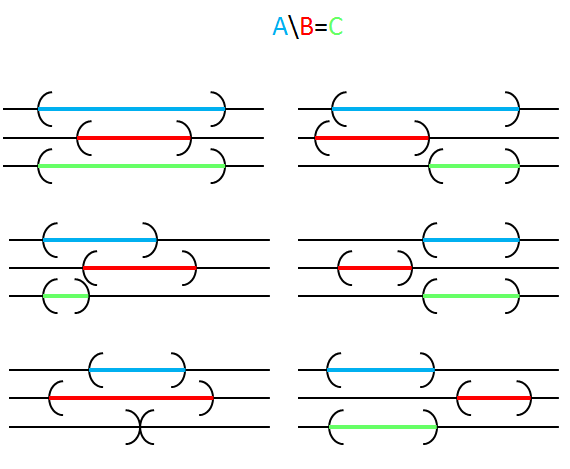
\includegraphics[width=150mm, keepaspectratio]{figures/aminusb.png}
	\caption{\label{fig:aminusb} Interval $A$ $\setminus$ Interval $B$ possible outcomes}
\end{figure}

\begin{definition}{Initial interval ($Ii$)=}
	
	An Interval where
	
	$LB$=$-\infty$
	
	$RB$=$+\infty$
	
	Initial interval $\equiv \Omega$ where $\Omega$ is the Full set of possible values
	
	($-\infty$,$+\infty$)
\end{definition}


\begin{definition}{complementer of an interval$ \overline{Interval}$=}
	
	$Ii \setminus Interval$
	
	ex.: $\overline{(2,8)}=(-\infty,+\infty)$ ($Ii$), $\overline{(-\infty,8)}=(9,+\infty)$, $\overline{Ei}=(Ii)$
\end{definition}

\begin{definition}{inside $k \in Interval$}
	
	let $k$ be $\in \mathbb{Z}$ and interval $Int$ be ($k$, $k$). then if $Int \cup Interval$ == $Int$ we say $k$ is inside $Interval$
	
	ex.: $7 \in (2,7)$
\end{definition}




%----------------------------------------------------------------------------
\section{Interval representation}
%---------------------------------------------------------------------------- 
\begin{definition}
Interval representation is a label for interval abstraction. It maps an interval to every variable. The possible values are inside the given intervals for every variable.
\end{definition}

\begin{theorem}	
	Let there be an Interval representation, where we map an Initial interval ($Ii$) to every variable. This interval representation is a good initial label for the abstraction analysis.
\end{theorem}

\begin{definition}
	Let there be an Interval representation. If every variable is mapped with a valid interval then we say the Interval Representation is .
\end{definition}

\begin{theorem}	
	Let there be two Interval representation $Ier1$ and $Ier2$ to the same program so it has the same variables. To every variable we map \[Ier1.IntervalforVar \cup Ier2.IntervalforVar\]This is a good $addLabel()$ function for the abstract analysis.
\end{theorem}
	
	{proof:} Let us say that this is not a good $addLabel()$ function. That means that exists a variable value that is allowed by one of the Interval representation, but is not allowed in \[Ier1.IntervalforVar \cup Ier2.IntervalforVar\] however this contradicts with the definition of the union of two intervals. So this should be a good $addLabel()$ function.	

%---------------------------------------------------------------------------
\section{No Partitioning Tactic<Interval representation>}
%---------------------------------------------------------------------------- 

\begin{definition}
	No Partitioning Tactic<Interval representation> is a Partitioning tactic for abstract analysis using Interval Representation as abstraction label.
\end{definition}

Every Partitioning Tactic should define how to set the target's label from a source's label and an edge's statement.

\begin{definition}
	Let there be an Interval $Interval$ and a statement $stmt$. Then we can apply $stmt$ to $Interval$ and it results in a new Interval. ($Interval.apply(stmt)$)
\end{definition}

Let there be a source's Interval representation $IerS$ and a statement $stmt$. No Partitioning Tactic<Interval representation> maps every variable to $IesS.IntervalforVar.apply(stmt)$.

\begin{theorem}
	Let there be an Interval $Interval$ for variable $var$ and a statement $stmt$. If $stmt$ has no effect on $var$ then
	$Interval.apply(stmt)=Interval$ 
\end{theorem}

{proof: } every possible values in the source location will be possible in the target location, and if a value is not allowed in the source location it will not be allowed in the target location since nothing has changed regarding the variable

\begin{theorem}
	Let there be an Interval $Interval$ for variable $var$ and a Skip statement $skipstmt$.It has no effect on the variable.
\end{theorem}
{proof: }it is directly comes from the definition of Skip statement. \hyperref[sec:cfaleiras]{see CFA section}

\begin{theorem}
	Let there be an Interval $Interval$ for variable $var$ and a Havoc statement $havstmt$. If $havstmt$ sets $var$ then
	$Interval.apply(havstmt)=Ii$. Otherwise it has no effect on the variable.
\end{theorem}

{proof: } if the statement sets the variable it means it can have any values. So we must represent the variable with $\Omega \equiv Ii$. Setting another variable does not have any effect on the current variable.


%---------------------------------------------------------------------------
\section{Applying Assign statement}
%---------------------------------------------------------------------------- 


\begin{definition}
	Let there be an Assign statement $assignstmt$. Then the interval that represents all the possible values allowed by the assignment is $assignstmt.transform$.
\end{definition}

\begin{theorem}
	Let there be an Interval $Interval$ for variable $var$ and an Assign statement $assignstmt$. If $assignstmt$ sets $var$ then
	$Interval.apply(assignstmt)=assignstmt.transform$. Otherwise it has no effect on the variable.
\end{theorem}
{proof: } if the statement sets the variable it means it will have the value given by the assignment. So we must represent the variable with the Interval that represents any values allowed by the assignment which is $assignstmt.transform$. Setting another variable does not have any effect on the current variable.

An assignment is made of Expressions. Using the Theta Framework \hyperref[sec:ref]{[4]} and considering only the integer type expressions the possibilities are as follows
\begin{itemize}
	\item Divide ($IntDivExpr$)
	\item Add ($IntAddExpr$)
	\item Subtract ($IntSubExpr$)
	\item Reference ($refExpr$) for variables.
	\item Literal ($IntLitExpr$) for literal expressions like 4 or 0
\end{itemize}

\begin{theorem}
	Let $k$ be a literal expression then the Interval that represents the possible values is $(k, k)$
\end{theorem}
{proof: } The only possible value is $k$

\begin{theorem}
	Let $Interval$ be a representation for possible values for variable $var$. Then a reference expression referencing $var$ can be represented with $interval$.
\end{theorem}
{proof: } The possible values are the same as it was before.

\begin{theorem}
	Let $EXpr1$, $EXpr2$, ... ,$EXprn$ be expressions represented by $Interval1$, $Interval2$, ..., $Intervaln$. then the Interval representation for $Add(EXpr1, EXpr2, ... ,EXprn)$ is
	
	if $Interval1.LB, Interval2.Lb, ... ,Intervaln.LB == -\infty$ then $result.LB=-\infty$
	else  $result.LB=\sum{Intervali.LB}$
	
	if $Interval1.HB, Interval2.Hb, ... ,Intervaln.HB == +\infty$ then $result.LB=+\infty$
	else  $result.LB=\sum{Intervali.HB}$
\end{theorem}
{proof: } the highest possible value is that every expression has the highest value. If all of them is finite then the biggest value is the sum of these, otherwise it is infinite. The lowest possible value is similar.

\begin{theorem}
	Let $EXpr1$, $EXpr2$ be expressions represented by $Interval1$, $Interval2$. Then the Interval representation for $Sub(EXpr1, EXpr2)$ is $result$ where:
	
	$result.LB=-\infty$ //initially
	
	$result.HB=+\infty$ //initially
	
	if $Interval1.HB \neq +\infty \land Interval2.LB \neq -\infty$ then 
	
	$result.HB=Interval1.HB-Interval2.LB$ ($Interval2.LB, Interval1.HB \in \mathbb{Z}$)
	
	if $Interval1.LB \neq -\infty \land Interval2.HB \neq \infty$ then 
	
	$result.LB=Interval1.LB-Interval2.HB$ ($Interval1.LB, Interval2.HB \in \mathbb{Z}$)
	
\end{theorem}
{proof: } Starting as every values will be possible. We can decide the maximum value by subtracting the lowest possible value from the highest possible value. Let the values be $a$ and $b$ where we want to calculate $a-b$ and $a, b \in \mathbb{Z}$ then $a-b>c-b$ if $a>c$ and $a-b>a-c$ if $b<c$. The lowest possible value is similar.


\begin{theorem}
	If we put more possible values to the assignment result we do not lose any possible values	
\end{theorem}
{proof: }If a value is possible and we put other possibilities as well, it is trivial that the original value will still be possible.

 Of course we might have some values that is incorrect, however as said in \hyperref[sec:partition]{the SAAI chapter} it is tolerable to say that something is reachable even though it is not. 

\begin{theorem}
	Let $EXpr1$, $EXpr2$ be expressions represented by $Interval1$, $Interval2$. Then the Interval representation for $Div(EXpr1, EXpr2)$ is 
	
	if $Interval1.LB \neq -\infty \land Interval1.HB \neq +\infty$ then 
	
		$A = $max( $|Interval1.LB|$ , $|Interval1.HB|$ )
	
		if($0$ is inside $Interval2$) then $B = 1$		
	
		else $B = $min( $|Interval1.LB|$ , $|Interval1.HB|$ )		
		
		$Div(EXpr1, EXpr2).HB = A/B$
		
		$Div(EXpr1, EXpr2).LB = -A/B$
		
	else
	
		$Div(EXpr1, EXpr2) = Ii$
	
\end{theorem}
{proof: } We simplify the problem by omitting the signs of the Bounds. This helps in the problem of sign changes (like (+)/(-)=(-)).  We do not lose any possible values since we search for the highest possible absolute value and the interval will be $(-highest, highest)$. Now if $Interval1$ biggest absolute value is infinite then the result will be infinite as well. ($\infty / a = \infty)$ If it is finite then let as consider $a$ and $b$ where $a, b \in \mathbb{Z}^{+}$.Then $a/b > c/b$ if $a>c$ and $a/b > a/c$ if $b<c$. So in $Interval1$ we search for the highest possible absolute value in $Interval2$ for the lowest possible value. If $interval2$ is just positive or negative then the the lowest absolute value is on the bound, otherwise it contains 0. Zero division is not allowed, however our abstraction sometimes put 0 into the possibilities even though it is not possible. (For instance after division we always put 0 in the possible values, however it is only possible if the dividend is zero) So if we omit the 0 value then the next smallest absolute value is 1.

\begin{theorem}
	Let $EXpr1$, $EXpr2$, ... ,$EXprn$ be expressions represented by $Interval1$, $Interval2$, ..., $Intervaln$. then the Interval representation for $Mul(EXpr1, EXpr2, ... ,EXprn)$ is
	
	if $Interval1.LB, Interval2.Lb, ... ,Intervaln.LB == -\infty \lor +\infty$ then 
	
	$Mul(EXpr1, EXpr2, ... ,EXprn)=Ii$
	
	else
	
	$Mul(EXpr1, EXpr2, ... ,EXprn)= \Pi $max($|Intervali.LB|$, $|Intervali.HB|$)
\end{theorem}
{proof: } We simplify the problem by omitting the signs of the Bounds. This helps in the problem of sign changes (like (+)/(-)=(-)).  We do not lose any possible values, because we search for the highest possible absolute value and the interval will be $(-highest, highest)$, so we only add more values. The biggest possible absolute value is when every multiplier has its highest possible value. If any multiplier is $\infty$ then the result is of course $Ii$


%---------------------------------------------------------------------------
\section{Applying Assume statement}
%---------------------------------------------------------------------------- 

\begin{definition}
	Let there be an Assume statement $assumestmt$ and a variable $var$. Then the interval that represents the values where the assumption is feasible for $var$ is $assumestmt.transform$.
\end{definition}

\begin{theorem}
	Let there be an Interval $Interval$ for variable $var$ and an Assume statement $assumestmt$. If $assumestmt$ has a condition to $var$ then
	$Interval.apply(assumestmt)=assumestmt.transform$. Otherwise it has no effect on the variable.
\end{theorem}
{proof: } If the statement has condition for the variable it means it will have the value allowed by the assumption. So we must represent the variable with the Interval that represents any possible values in the assumption which is $assumestmt.transform$.

\begin{theorem}
	An Assume statement can only narrow down the possible values.
\end{theorem} 
{proof: } If a value is not allowed in the source location, then it will not be possible in the target location since we, do not change the variable

The consequence of this theorem is this next theorem:
\begin{theorem}
	Let there be an Interval $Interval$ for variable $var$ and an Assume statement $assumestmt$. We do not lose any possible values if $Interval.apply(assumestmt)=Interval$
\end{theorem} 

\begin{definition}
	A $condition$ is an interval, which represents the possible values for a variable (can be calculated from any Expression used in the assignment).
\end{definition}

\begin{definition}
	We say an assumption is trivial for a variable $var$ if it is in a form of: $var \{==, \neq, \geq, >, \leq, < \} condition$ where $condition$ is an interval (it can be calculated from any Expression used in the assignment, but shall not depend on $var$)
\end{definition}

\begin{definition}
	Let variable $var$ be represented by $interval$. An incorrect value is inside $interval$,  but $var$ is not allowed to have this value.
\end{definition}

\begin{definition}
	An incorrect condition is a $condition$, which is an interval that may have incorrect values.
\end{definition}

\begin{theorem}
	A trivial condition is then and only then incorrect, if the $condition$ is calculated using reference, multiply or divide expression
\end{theorem} 
{proof: } then:

 Reference expression can be represented by an interval for a variable, which allows incorrect values.
 
 Multiply, and divide expression both uses over exaggeration for the possible values.
 
 only then: all the other possible assignments allow only the possible values. 

\begin{definition}
	We say an Assume statement is applicable for a variable if the statement consists of $AND$, $OR$ or $NOT$ functions of a trivial assumption for the variable. It is not applicable though if the Assume statement has incorrect condition.
\end{definition}

Let there be an Interval $Interval$ for variable $var$ and an Assume statement $assumestmt$. if $assumestmt$ is not applicable $assumestmt.transform = Interval$. We can do this because of Theorem 17


\begin{theorem}
	Let there be a trivial assumption for variable $var$ represented by $IntervalVar$ where the assumption's $condition$ is correct and represented by $IntervalCondition$
	
	then
	
	$var \geq condition=($max($IntervalCondition.LB$, $IntervalVar.LB$),$IntervalVar.HB)$
	
	ex. $(3, 7) \geq (1,5) = (3,7)$, $(3, 7) \geq (5,5) = (5,7)$
	
	$var \leq condition=(IntervalVar.LB$, min($IntervalCondition.HB$, $IntervalVar.HB))$
	
	ex. $(3, 7) \leq (1,5) = (3,5)$, $(3, 7) \leq (1,1) = (3,1) \equiv Ei$
	
	$var > condition=($max($IntervalCondition.LB+1$, $IntervalVar.LB$),$IntervalVar.HB)$
	
	ex. $(3, 7) > (3,5) = (4,7)$, $(3, 7) > (2,5) = (3,7)$
	
	$var < condition=(IntervalVar.LB$, min($IntervalCondition.HB-1$, $IntervalVar.HB))$
	
	ex. $(3, 7) < (1,5) = (3,4)$, $(3, 7) < (3,3) = (3,2) \equiv Ei$
	
	$var \neq condition=var \setminus condition$
	
	ex.  $(3, 7) \neq (1,5) = (6,7)$, $(6, 7) \neq (1,5) = (6,7)$
	
	$var == condition = var \cup condition$
	
	ex.  $(3, 7) == (1,5) = (1,5)$, $(6, 7) == (1,5) = Ei$
	
	Note: $\neq$ is the only one that can make incorrect possible values. For example $(3, 7) \neq (4,5) = (3,7)$ however $4$ and $5$ are incorrect. Still we only allow more possibilities.
	
\end{theorem}
{proof: } $<, >$: Let $var > condition$ be $(a, b)>(c, d)$ and valid then $var > condition=(max(a, c+1), b)$ 

if $a>c+1$ then

 $\forall i \in (a, b), \exists j \in (c, d)$ where $ i>j$ so it is true and 
 
 $\forall i \notin (a, +\infty), \nexists j \in (a, b)$ where $ i>j$ 
 
 $\forall i \notin (-\infty, b), \nexists  i<b$ no incorrect possible value is added
 
 else  $\forall i \in (c+1, b), \exists j \in (c, d)$ where $ i>j$ so it is true and
 
 $\forall i \notin (c+1, +\infty), \nexists j \in (c, b)$ where $ i>j$ 
 
 $\forall i \notin (-\infty, b), \nexists  i<b$ no incorrect possible value is added
 
 The other equation can be similarly proved.

\begin{definition}
	If an Assume statement consists of $AND$ functions of trivial assumption and the trivial assumptions result intervals are $Interval1, Interval2, ..., Intervaln$, then $assumestmt.transform = Interval1 \cap Interval2 \cap ... \cap Intervaln $
\end{definition} 

\begin{theorem}
	The previously defined result interval is correct (has all the possible values)
\end{theorem}
{proof: } The assumption is true only if every operant is true. An operant is true if the value is inside the interval that represents the operand so the section of these intervals is the possible values. Let us say there is a value where the result should be true, but it is not in the section. Then it is only not in the section, because one interval does not allow it. That operant results in false to this value thus the overall result will be false. So the value must be in the section.

Note: The operants does allow all the possible values (only $\neq$ can allow incorrectly values, but still allows the correct ones)

\begin{definition}
	If an Assume statement consists of $OR$ functions of trivial assumption and the trivial assumptions result intervals are $Interval1, Interval2, ..., Intervaln$, then $assumestmt.transform = Interval1 \cup Interval2 \cup ... \cup Intervaln $
\end{definition} 

\begin{theorem}
	The previously defined result interval is correct (has all the possible values)
\end{theorem}
{proof: } The assumption is false only if every operant is false. An operant is false if the value is not inside the interval that represents the operand. Let us say there is a value where the result should be true, but it is not in the union. It is only possible if the value is not inside of any operants interval. So all operants results in false for the value thus the overall result will be false. So the value must be in the union.

Note: The operants does allow all the possible values (only $\neq$ can allow incorrectly values, but still allows the correct ones)

\begin{definition}
	If an Assume statement consists of a $NOT$ function and is similar $Not(condition)$ and the $condition$ was calculated with allowing no incorrect values and $IntervalCondition$ is the interval representation for $condition$ and we search for the new interval of a variable represented previously by $IntervalVar$ then $Not(condition)=IntervalVar \setminus condition$
\end{definition} 

\begin{theorem}
	The previously defined result interval is correct (has all the possible values)
\end{theorem}
{proof: } The assumption is true only if the condition is false.The Condition is false if the value is not inside the interval that represents the condition. Let us say there is a value where the result should be true, but it is not in $IntervalVar \setminus condition$. It is only possible if the value is inside of $condition$. Note: it must be inside $IntervalVar$. So the condition results in true for the value thus the overall result will be false. Note: if the $condition$ interval has values that should be resulted in false, than these values overall result should be true, therefore $condition$ should not allow incorrect values. So the value must be in $Ii \setminus condition$.

Note: This can also allow incorrect values, but at least allows all the possible ones.

\begin{theorem}
	if we allow $condition$ to be calculated by not only the assignment statements ($ADD$, $MUL$, etc). but conditional statements as well ($\geq$, $AND$, etc).Then $condition$ is then and only then correct, when $condition$ is calculated using no reference, multiply, divide, $\neq$ or $NOT$ expression
\end{theorem}
{proof: } We already discussed reference, multiply and divide. $\neq$ or $NOT$ is similar to it since these can allow incorrect values.

%----------------------------------------------------------------------------
\section{Possible partitions}
%---------------------------------------------------------------------------- 

In some cases we allowed incorrect values for an interval. A trivial example is $a \neq 0$. in this case we set the interval for $a$ to $Ii$ thus having $0$ as an incorrect value. One partitioning tactic could be to cat the result intervals to more pieces so we can have gaps as well.

For the previous example we can represent the possible values by two intervals $(-\infty, -1)$ and $(1, \infty)$.

This would make it possible to make $\neq$ a usable function in correct $condition$s.

In this case the label for a location could be mapping every variable to a set of intervals (not just one interval)

%---------------------------------------------------------------------------
\section{No Widening Tactic<Interval representation>}
%---------------------------------------------------------------------------- 

\begin{definition}
	No Widening Tactic<Interval representation> is a Widening tactic for abstract analysis using Interval Representation as abstraction label.
\end{definition}

Every Widening Tactic should define how to set the target's label from a source's label, an edge's statement and the target's previous label.

\begin{theorem}
	Let the target's new Interval be $IntervalNew$ and the previous be $IntervalOld$, then $\forall i \in IntervalOld$ it is true that $i \in  IntervalNew$.
\end{theorem}
{proof: } "If a location is reached and labeled, than its new label can only be less specific." \hyperref[sec:cfaalgorithm]{see previous chapter}

Let there be a source's Interval representation $IerS$, targets previous interval representation $IerT$ and a statement $stmt$. No Widening Tactic<Interval representation> maps every variable to $IerT \cup IesS.IntervalforVar.apply(stmt)$.

\begin{theorem}
	The above mentioned tactic results in no loss of possible values
\end{theorem}
{proof: } Let us say value $a$ should be possible in the target location, but $a \notin IerT \cup IesS.IntervalforVar.apply(stmt)$. This means $a \notin IesS.IntervalforVar.apply(stmt) \land a \notin Ier$. $IesS.IntervalforVar.apply(stmt)$ allows all the possible new values (see previous sections). So $a$ can not be a new value so it has to be an old one, but we said $a \notin Ier$. So every possible value is still possible
 

%---------------------------------------------------------------------------
\section{Other possible Widening Tactic}
%---------------------------------------------------------------------------- 

Let $interval = (0,0)$ be the representation for a variable in a certain location. Assume there is an edge, which increments the variable by one. After applying the statement of this edge the new interval will be $interval = (0, 1)$. Assuming that this edge' source always changing (for example the source location is the same as the target) then $interval.HB$ can increase infinitely.

One possible solution for this problem is a widening tactic which actually has some widening approach.

Let there be a location, which is already labeled, with an interval representation. Let $intervalOld$ be an interval mapped for variable $a$. After the label is "refreshed" (this location was the target in a modifying edge.) let $intervalNew$ be an interval mapped for variable $a$. If $\exists i$ where $i \in intervalNew \land i \notin intervalOld$ We can say that the label for this location "wider".

To eliminate the possibility to widen the label infinitely, after one widening we change the label to prevent further widening. In the interval it can be for example the previously mentioned $(0, 0), (0,1), (0,2), ...$ can be prevented by instead of mapping tha variable with $(0,1)$ we immediately map it with $(0, +\infty)$.

To prevent allowing too many incorrect values, we have to make it possible, to narrow the previously widened label.

For instance in the previous example, there can be an assumption that the variable must be smaller than $7$. In this case we can narrow the widened interval $(0,+\infty)$ to $ (0, 7)$.


%---------------------------------------------------------------------------
\section{Abstracted information}
%---------------------------------------------------------------------------- 

Abstraction always means that some information will inevitably get lost. Using Interval representation as labels for the location also has information losses.

During No Partition tactic we allowed that the intervals can represent incorrect values as long as it represents all the correct (possible) values. This already is some lost information.

Another even bigger concern that we lose some major connection between variables. Since every variable is maintained independently from the others. Let there be two variables $var1, var2$. There could be a correlation such that in a location $var1=1$ if $var2=1$ and $var1=0$ otherwise. The above described interval representation would label this: $var1 \in (0, 1) var2 \in (-\infty, +\infty)$. So we lost the information that $var1$ is only $1$ if $var2=1$. Fortunately this problem only widens the possible values.